%	JASA LaTeX Sample File, Preprint Sample
%
%  Beginner Latex users should refer to their favorite online documentation
%  here is one from the TeX Users Group 
%	https://www.tug.org/twg/mactex/tutorials/ltxprimer-1.0.pdf
%
%  Useful FAQ from  https://journals.aps.org/revtex/revtex-faq
% 

%%%%%%% For Preprint
%% For manuscript, 12pt, one column style

\documentclass[dvipsnames, reprint]{JASA}
\usepackage[pdftex]{}
\graphicspath{{figures/}}
\usepackage[dvips]{epsfig,graphicx}
\DeclareGraphicsExtensions{.pdf,.jpeg,.png, .eps}

\usepackage{xcolor}
\def\SBcomment[#1]{\tex tcolor{Red}{#1}}
\def\SWcomment[#1]{\textcolor{Bittersweet}{#1}}
\def\MDcomment[#1]{\textcolor{Blue}{#1}}
\def\SScomment[#1]{\textcolor{OliveGreen}{#1}}

%%%%% Preprint Options %%%%%
%% The track changes option allows you to mark changes
%% and will produce a list of changes, their line number
%% and page number at the end of the article.
 %\documentclass[preprint,trackchanges]{JASA}


%% NumberedRefs is used for numbered bibliography and citations.
%% Default is Author-Year style.
% \documentclass[preprint,NumberedRefs]{JASA}

%%%%%%% For Reprint
%% For appearance of finished article; 2 columns, 10 pt fonts

% \documentclass[reprint]{JASA}

%%%%% Reprint Options %%%%%

%% For testing to see if author has exceeded page length request, use 12pt option
% \documentclass[reprint,12pt]{JASA}


%% NumberedRefs is used for numbered bibliography and citations.
%% Default is Author-Year style.
% \documentclass[reprint,NumberedRefs]{JASA}

%% TurnOnLineNumbers
%% Make lines be numbered in reprint style:
% \documentclass[reprint,TurnOnLineNumbers]{JASA}

%% Optional algorithm package. You can comment this out and
%% include another package if you prefer another way to make
%% algorithms examples (but please check that the package is compatible with 
%%Editorial Manager; see JASA-EL-TeXGuide.pdf).


\usepackage{algpseudocode}

\begin{document}

\title[JASA/Dynamic Grids for Finite-Difference Schemes]{Dynamic Grids for Finite-Difference Schemes: Changing Parameters of Musical Instrument Simulations in Real Time}
\author{Silvin Willemsen}
\email{sil@create.aau.dk}
\author{Stefania Serafin}
\affiliation{Multisensory Experience Lab, CREATE, Aalborg University, Copenhagen, Denmark}

\author{Stefan Bilbao}
\affiliation{Acoustics and Audio Group, University of Edinburgh, Edinburgh, Scotland}
 
% \author{Author Five}			
% \altaffiliation{Also at: Department, University, City, State ZipCode, Country.}
% \affiliation{Department3,  University3, City, State ZipCode, Country}


\preprint{Willemsen, JASA}		%  if you want want this message to appear in upper right corner of title page

\date{\today} 

\begin{abstract}
Simulating musical instruments using physical modelling is a well-established field. Among the reasons of why one would simulate an instrument rather than sample an existing one, is that one could extend the capabilities of this instrument beyond what is physically possible, such as changing material properties or size of the instrument on the fly. Many modelling techniques exist of which finite-difference time-domain (FDTD) methods are considered the most flexible and generalisable in terms of the type of systems they can model, both linear and nonlinear. These methods do, however, lack the capability of handling smooth parameter changes while retaining optimal simulation quality, something other techniques are better suited for. This article proposes a method to dynamically alter the grids of simulations based on FDTD methods by smoothly adding and removing grid points from the system, which allows for dynamic parameter changes in physical models of musical instruments which are based on this technique. Furthermore, this technique allows the stability condition that the schemes using FDTD methods are based on, to always be satisfied with equality and thus have the highest simulation quality possible. 
\end{abstract}

%% pacs numbers not used

\maketitle

%  End of title page for Preprint option --------------------------------- %



\section{\label{sec:introduction} Introduction}
Simulation of musical instruments through physical modelling is a well established field... 
\SWcomment[Much more intro here obviously]{}
% of simulating musical instruments rather than recording them and playing them back (samples), is the flexibility of control and playability of the instrument. Imagine trying to record the entire control space of a violin, i.e., all possible combinations of bowing force, bowing velocity and fingering positions. The recording procedure would take a great amount of time and resources, let alone the amount of data storage required to store all of the high-quality audio.

% Due to the vast parameter space of many instruments, using simulations is a much more viable solution for capturing the full expressivity of an instrument than sampling.


One of the incentives of simulating the physics of musical instruments rather than recording their real-world counterparts, is that the virtual instrument can be manipulated in physically impossible ways. Examples of this could be to change material properties, or even the shape of the instrument on the fly. An example of a real-world instrument that requires these manipulations is the trombone, where tube-length needs to be dynamic in order to play the instrument. \SWcomment[In a companion article the authors describe a physical model of this instrument as a case study for the techniques presented here.] 

% This can be extended from musical instruments to rooms and acoustic simulation with variable shapes

Existing physical modelling techniques include mass-spring systems [REF] and digital waveguides [REF]. Modal synthesis [REF], though requiring some assumptions and simplifications for most systems, does allow for easy and smooth parameter changes -- as seen in [REF] and [REF] -- and could thus be a good candidate for implementing the aforementioned manipulations. \SWcomment[In the case of the trombone, and due to its non-homogenous geometry, there is no closed-form solution available and the modes would need to be calculated for every single slide configuration.] Finite-difference time domain (FDTD) methods on the other hand, though generally more computationally expensive than other techniques, are more flexible and generalisable and do not need as many simplifications as modal synthesis does. These methods subdivide continuous partial differential equations (PDEs) that describe the physics of the system at hand into a grid of discrete points in space and time. 
%
% Below, a brief introduction about grids and their relationship to stability is explained.
%
% \subsection{Grids and stability}
The distance between two discrete points in space (the grid spacing) and the time step between two discrete moments in time are closely connected through a \textit{stability condition}. This condition dictates the maximum number of points allowed to describe system before it gets unstable and the simulation ``explodes''. The closer the grid spacing is to the stability condition, the higher the quality of the simulation. If the condition is satisfied with equality, the quality of the simulation is at a maximum. 
Furthermore, the stability condition depends on the parameters of the model, such as material properties or size of the system, i.e., parameters that could be changed on the fly.

This article proposes a method to smoothly add and subtract points from a system in real time so that the stability condition is always satisfied with equality. This allows for a simulation where the parameters can be changed dynamically without running into either stability or quality issues. 

This article is structured as follows: 
\textit{NOTES:}
\begin{itemize}
% \item Section 2: Background on PDE $\rightarrow$ FDTD $\rightarrow$ stability conditions 
\item Section 2: Continuous systems
\item Section 3: Numerical methods
\item Section 4: Dynamic grid
\item Section 5: Results
\item Section 6: Discussion
\item Section 7: Conclusions and Future work
\end{itemize}
\section{Continuous Systems}\label{sec:continuous}
%
%going from a partial differential equation (PDE) to an update equation that can be implemented.
%
%using the famous 1D wave equation.
%
The physics of dynamic systems is commonly described using partial differential equations (PDEs) operating in continuous time. To aid the illustration of the proposed method, the 1D wave equation will be used. \SWcomment[This does not mean that the method is limited to this, and could be extended to other (linear) systems, even higher dimensional ones.]

Consider a 1-dimensional system with length $L$ (in m) described by state variable $u = u(x, t)$ defined over spatial domain $x \in [0, L]$ (in m) and time $t \geq 0$ (in s). The partial differential equation (PDE) of the 1D wave equation is then described as
\begin{equation}\label{eq:1dwave}
    \frac{\partial^2 u}{\partial t^2}= c^2\frac{\partial^2 u}{\partial x^2}\ ,
\end{equation}
parameterised by wave speed $c$ (in m/s). As $x$ in Eq. \eqref{eq:1dwave} is only defined over a finite region in space, boundary conditions need to be provided. Two possible conditions are
\begin{subequations}\label{eq:continuousBoundaries}
    \begin{align}
        u(0, t) = u(L, t) &= 0\quad \text{(Dirichlet)},\label{eq:contDirichlet}\\
        \frac{\partial}{\partial x} u(0, t) = \frac{\partial}{\partial x} u(L, t) &= 0\quad \text{(Neumann)},\label{eq:contNeumann}
    \end{align}
\end{subequations}
which describe a `fixed' and `free' boundary respectively.

\subsection{Dynamic parameters}
In the case of the 1D wave equation, only the wave speed $c$ and length $L$ can be altered. If Dirichlet-type boundary conditions -- as in Eq. \eqref{eq:contDirichlet} -- are used, the fundamental frequency $f_0$ of the 1D wave equation can be calculated according to
\begin{equation}\label{eq:fundamentalFreq}
    f_0 = \frac{c}{2L}\,.
\end{equation}
From Eq. \eqref{eq:fundamentalFreq}, one can easily conclude that, in terms of fundamental frequency halving the length of Eq. \eqref{eq:1dwave} is identical to doubling the wave speed and vice versa. Looking at system \eqref{eq:1dwave} in isolation, $f_0$ is the only behaviour of the system that can be changed. One can thus leave $L$ fixed %($L = 1$ for simplicity) 
and make $c$ dynamic (or time-varying), i.e., $c = c(t)$, which will prove easier to work with in the following section.

\section{Numerical methods}\label{sec:FDTD}
This section will give a brief introduction of physical modelling using FDTD methods, including details on stability and quality of the simulations based on these methods.

\subsection{Discretisation}
Using FDTD methods, the continuous 1D wave equation in Eq. \eqref{eq:1dwave} can be discretised into points in space and time. The spatial variable can be discretised using $x_l = lh$ (read: $x$ at location $l$) with integer $l \in [0, \hdots, N]$, grid spacing (distance between two consecutive grid points) $h$ (in m) and total number of points $N + 1$ (including the boundaries) where
\begin{equation}\label{eq:numberOfPoints}
    N = \text{floor}(L/h),
\end{equation}
is the total number of intervals between the grid points. The temporal variable can be discretised using $t_n = nk$ with positive integer $n$, time step $k = 1/f_\text{s}$ (in s) and sample rate $f_\text{s}$ (in Hz). The state variable $u$ can then be approximated using $u(x,t) \approx u_l^n$, where grid function $u_l^n$ is ``the state $u$ at spatial index $l$ and time index $n$". The total state at time index $n$ is then denoted as vector $\mathbf{u}^n$ with size $N+1$.

The following operators can then be applied to $u_l^n$ to get the following approximations to the derivatives in Eq. \eqref{eq:1dwave}
\begin{subequations}\label{eq:operators}
    \begin{align}
         \delta_{tt}u_l^n &= \frac{1}{k^2}\left(u_l^{n+1}-2u_l^n + u_l^{n-1}\right)\;\;\approx\quad\frac{\partial^2u}{\partial t^2}\label{eq:secondOrderTime}\ ,\\
         \delta_{xx}u_l^n &= \frac{1}{h^2}\left(u_{l+1}^n-2u_l^n + u_{l-1}^n\right)\quad\approx\quad \frac{\partial^2u}{\partial x^2}\ .\label{eq:secondOrderSpace}
    \end{align}
\end{subequations}
Substituting these definitions into Eq. \eqref{eq:1dwave} yields the following finite-difference scheme (FDS)
\begin{equation}\label{eq:FDS}
    \delta_{tt}u_l^n = c^2 \delta_{xx}u_l^n.
\end{equation}
Expanding the operators as in %the Eqs. in
\eqref{eq:operators} and solving for $u_l^{n+1}$ (which is the only unknown) yields the following update equation
\begin{equation}\label{eq:updateEq}
    u_l^{n+1} = 2u_l^n-u_l^{n-1} + \lambda^2 \left(u_{l+1}^n-2u_l^n + u_{l-1}^n\right),
\end{equation}
saying that $u$ at the next time index ($n+1$) can be calculated using only values of $u$ at the current ($n$) and previous time indices ($n-1$). \SWcomment[This update can be implemented in software, such as {\tt MATLAB} or {\tt C++}.] Here, $\lambda = ck/h$ is referred to as the Courant number and determines whether the system is stable, as well as the quality and behaviour of the simulation. This will be described in detail in Sections \ref{sec:stability} and \ref{sec:quality}.

In the FDS described in Eq. \eqref{eq:FDS}, the boundary locations are at $l = 0$ and $l = N$. Substituting these locations into Eq. \eqref{eq:updateEq} seemingly shows that grid points outside of the defined domain are needed, namely $u_{-1}^n$ and $u_{N+1}^n$. These can be referred to as \textit{virtual grid points} and can be accounted for %/defined
by using the boundary conditions in Eq. \eqref{eq:continuousBoundaries}. Discretising these yields
\begin{subequations}
    \begin{align}
        u_0^n = u_N^n &= 0 \quad\text{(Dirichlet)}\label{eq:discreteDirichlet}\\
        \delta_{x\cdot} u_0^n = \delta_{x\cdot} u_N^n &= 0 \quad \text{(Neumann)}\label{eq:discreteNeumann}
    \end{align}
\end{subequations}
where 
\begin{equation}
    \frac{\partial u}{\partial x} \approx \delta_{x\cdot}u_l^n = \frac{1}{2h}\left(u_{l+1}^n - u_{l-1}^n\right)
\end{equation}
is a second-order accurate approximation of the first-order spatial derivative. The Dirichlet condition in \eqref{eq:discreteDirichlet} says that the states at the boundary locations are always 0. In practice, this means that these grid points do not need to be updated and the spatial range of calculation for Eq. \eqref{eq:updateEq} then becomes $l = [1, \hdots, N-1]$. If the Neumann condition is used, the boundary points do need to be updated as these are not necessarily $0$; rather, their `slope' is $0$. Eq. \eqref{eq:discreteNeumann} can then be expanded to yield defnitions for these virtual grid points
\begin{equation}\label{eq:neumannSolution}
    u_{-1}^n = u_1^n \quad \text{and} \quad u_{N+1}^n = u_{N-1}^n\,.
\end{equation}

Now that the full system is described the output sound can be retrieved by following the state $u_l^n$ in Eq. \eqref{eq:updateEq} at $0 < l < N$ (when using fixed boundary conditions \SWcomment[, unless silence is your thing]) and listening to that at the given sample rate $f_\text{s}$.

\subsection{Stability}\label{sec:stability}
Discretising continuous equations using numerical methods place limits on the parameters describing it. A wrong choice of parameters could render the system unstable and make it ``explode". In the case of the update in Eq. \eqref{eq:updateEq} it can be shown -- using Von Neumann stability analysis [REF] -- that the system is stable if
\begin{equation}\label{eq:CFL}
    \lambda \leq 1,
\end{equation}
referred to as the Courant-Friedrichs-Lewy (CFL) stability condition. The closer $\lambda$ is to this condition, the higher the quality of the simulation (see Section \ref{sec:quality}) and if $\lambda = 1$, Eq. \eqref{eq:updateEq} provides an exact solution to Eq. \eqref{eq:1dwave} %(this is true for the 1D wave equation)
[REF] (see Figures \ref{fig:lambda1} and \ref{fig:lambda0.9}). If $\lambda > 1$ the system will become unstable (see Figure \ref{fig:lambda1.001}).
\begin{figure*}
\figline{\fig{ulnLambda1}{.25\textwidth}{(A)}\label{fig:lambda1}
\fig{ulnLambda0.9}{.25\textwidth}{(B)}\label{fig:lambda0.9}
\fig{ulnLambda1001}{.25\textwidth}{(C)}\label{fig:lambda1.001}
\narrowcaption{.25\textwidth}{State $u_l^n$ with $N = 50$ and $f_\text{s} = 44100$ visualised. (A) If $\lambda = 1$, the solution is exact. (B) If $\lambda < 1$ dispersive behaviour shows. (C) If $\lambda > 1$ the CFL condition in Eq. \eqref{eq:CFL} is not satisfied and the system ``explodes".
\label{fig:dispersion}}}
\end{figure*}
% discrete boundaries here?
One can rewrite Eq. \eqref{eq:CFL} in terms of grid spacing $h$ to get
\begin{equation}\label{eq:stabilityCond}
    h \geq ck.
\end{equation}
This shows that the CFL condition in \eqref{eq:CFL} puts a lower bound on the grid spacing, calculated from the sample rate and wave speed. Usually, the following steps are taken to calculate $\lambda$
\begin{equation}\label{eq:orderOfCalcGrid}
    h := ck,\ \ N := \text{floor}(L/h), \ \ h := L/N, \ \ \lambda := \frac{ck}{h}.
\end{equation}
In other words, condition \eqref{eq:stabilityCond} is first satisfied with equality and used to calculate integer $N$ according to Eq. \eqref{eq:numberOfPoints}. Thereafter, $h$ is recalculated based on $N$ and used to calculate $\lambda$. The calculation of $\lambda$ in Eq. \eqref{eq:orderOfCalcGrid} can be compactly rewritten as
\begin{equation}\label{eq:compactLambda}
    \lambda = \frac{ck}{L}\cdot\text{floor}\left(\frac{L}{ck}\right).
\end{equation}
The flooring operation causes the CFL condition in \eqref{eq:CFL} to not always be satisfied with equality and results in a reduced simulation quality described in the following section.

\subsection{Simulation Quality}\label{sec:quality}
As mentioned above, the Courant number $\lambda$ decides the quality of the simulation. Choosing $\lambda < 1$ will decrease this quality in two ways. Firstly, it will decrease the maximum frequency that the simulation is able to produce, i.e., it will decrease the bandwidth of the output sound of the system. See Figure \ref{fig:bandWidths}.
%
\begin{figure*}
\figline{\fig{bandwidthLambda1}{.25\textwidth}{(A)}
\fig{bandwidthLambda0.9}{.25\textwidth}{(B)}
\fig{bandwidthLambda0.5}{.25\textwidth}{(C)}
\narrowcaption{.25\textwidth}{Bandwidths of the simulation output %at $l = 16$ 
with $f_\text{s} = 44100$ Hz and 
%$N = 50$ excited with a raised cosine with a width of 5 at center-location $N = 25$. The Courant number is set to 
(A) $\lambda = 1$, (B) $\lambda = 0.9$ and (C) $\lambda = 0.5$. 
\label{fig:bandWidths}}}
\end{figure*}
%
By analysing the scheme in Eq. \eqref{eq:updateEq}, it can be shown that the maximum frequency produced by the system can be calculated using \cite[Chap. 6]{bilbao2009}
\begin{equation}\label{eq:fmax}
    f_\text{max} = \frac{f_\text{s}}{\pi} \sin^{-1}(\lambda),
\end{equation}
shown in Figure \ref{fig:bandWidthFormula}.
%
Note that only a small deviation of $\lambda$ from condition \eqref{eq:CFL} already has a profound effect on the bandwidth of the output.

\begin{figure}
%% \reprintcolumnwidth is the same in preprint and reprint for
%% ease of use for authors:
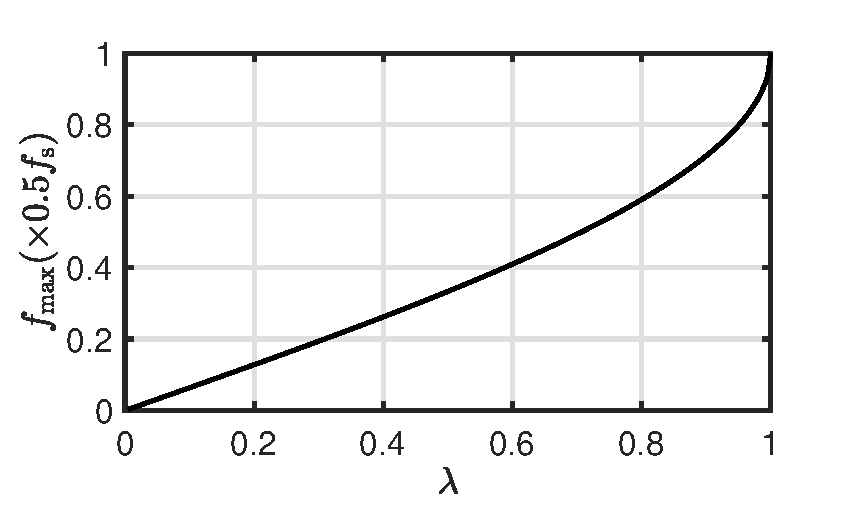
\includegraphics[width=0.8\reprintcolumnwidth]{bandwidthPlot}
\caption{\label{fig:bandWidthFormula}{The effect of the Courant number $\lambda$ on the output bandwidth. \SWcomment[This figure should probably be much more compact, if not removed altogether.]}}
\end{figure} 

Secondly, choosing $\lambda < 1$ causes numerical dispersion. See Figures \ref{fig:lambda0.9} and \ref{fig:bandWidths}. Harmonic partials get closer together at higher frequencies (i.e. get more inharmonic) as $\lambda$ decreases, which is generally undesirable.

Apart from the recalculation of $\lambda$ due to the flooring operation in Eq. \eqref{eq:orderOfCalcGrid}, a reason that one would choose $\lambda < 1$ could be to decrease the total number of grid points used in the simulation by increasing $h$. This makes the simulation less computationally expensive, while keeping a desired wave speed $c$ and time step $k$. For 1-dimensional systems, such as the 1D wave equation, this is rarely necessary.

\section{Dynamic Parameters}
This section describes how parameters could be made dynamic using the state of the art and what this means for the simulation quality detailed in Section \ref{sec:quality}. %To clarify, for a parameter to be dynamic refers to its ability to vary over time while the simulation is running.  
To clarify, a \textit{dynamic} parameter refers to one that is time-varying while the simulation is running. 

% For the 1D wave equation used in Section \ref{sec:FDTD}, a property that could be interesting to make time-varying is the fundamental frequency $f_0$. If Dirichlet-type boundary conditions are used, as defined in Eqs. \eqref{eq:contDirichlet} and \eqref{eq:discreteDirichlet}, $f_0$ can be calculated according to
% \begin{equation}\label{eq:fundamentalFreq}
%     f_0 = \frac{c}{2L}\,.
% \end{equation}
% If $\lambda = 1$ in \eqref{eq:CFL} and thus condition \eqref{eq:stabilityCond} is satisfied with equality, $L/h$ in Eq. \eqref{eq:numberOfPoints} is an integer and the flooring operation can be ignored. Substituting \eqref{eq:numberOfPoints} into \eqref{eq:fundamentalFreq} yields
% \begin{equation}
%     f_0 = \frac{1}{2Nk}\ ,
% \end{equation}
% which shows that if $\lambda = 1$, $N$ solely decides the fundamental frequency of the simulation.

Usually when simulating instruments, the parameters that describe the system are fixed for the entire simulation. For the 1D wave equation used in Section \ref{sec:continuous}, these are the wave speed $c$ and time step $k$ (calculated from the sample rate $f_\text{s}$) from which the grid spacing $h$ and Courant number $\lambda$ are calculated. On top of this, the length $L$ can be changed, but as shown in Eq. \eqref{eq:fundamentalFreq}, this can be directly translated to a change in $c$ through the fundamental frequency $f_0$. As $f_\text{s}$ is rarely changed, the sole parameter that could be interesting to make time-varying is $c$. 
% Modal synthesis is based on the addition of many sinusoids and is thus defined over the entire space. One can simply change the frequency of these sinusoids and 

% \begin{equation}\label{eq:modalSum}
%     u(x,t) = \sum_{m=1}^M C_m\sin(\omega_mt+\phi_m)\sin\Big(\frac{m\pi x}{L}\Big),
% \end{equation}
%
% The amount of modes that can be included also depends on a stability condition, but it is much easier to work with. One simply excludes modes that do not satisfy this condition. 
%
% Using FDTD methods, one uses a discrete set number of points making it hard to transition from one setting to the next.

As the number of grid points hangs tightly together with these parameters, changing $c$ would mean a change in $N$ according to Eq. \eqref{eq:orderOfCalcGrid}. This raises questions as to \textit{where} and especially \textit{how} one would add and remove points to the grid according to the now-dynamic wave speed. To avoid this, one could set and fix the number of points of a discrete system and tune the parameters away from the stability condition, such as done in [REF]. As such, one could choose a wave speed $c$, set and fix $N$ at the beginning of the simulation and decrease the value of $c$. This would avoid problems with stability, as decreasing $c$ would continue to satisfy condition \eqref{eq:stabilityCond}, but the simulation would, however, end up with lower quality, exhibiting dispersive and bandlimiting effects as discussed in Section \ref{sec:quality}. In essence, decreasing the value of $c$ immediately translates to decreasing the value of $\lambda$ as $h$ and $k$ are left unchanged.

To implement a physical model with dynamic parameters and an optimal simulation quality at all times, a method needs to be devised to dynamically change the number of grid points.

% Section \ref{sec:quality} shows several arguments for why these parameters should be fixed. The stability of the simulation relies on the parameters of the scheme and needs to be satisfied as close to the condition  When the stability condition is calculated,

% In this case we could initialise the system to have a wave speed of $c = 300$ m/s and a sample rate of $f_\text{s} = 44100$ Hz yielding $N = 147$ and $lambda = 1$ (satisfying condition \eqref{eq:CFL} with equality.

% Essentially $c$ is made time-varying / dynamic / changed on the fly $c^n$
% \subsection{Connection between $c$ and $L$ \SWcomment[(might be better as an appendix)]}\label{sec:f0}
% If Dirichlet-type boundary conditions are used, as defined in Eqs. \eqref{eq:contDirichlet} and \eqref{eq:discreteDirichlet}, the fundamental frequency $f_0$ of the 1D wave equation can be calculated according to
% \begin{equation}
%     f_0 = \frac{c}{2L}\,,
% \end{equation}
% from which one can see that, in terms of fundamental frequency a halving the length is identical to doubling the wave speed. 
% If $\lambda = 1$ in \eqref{eq:CFL} and thus condition \eqref{eq:stabilityCond} is satisfied with equality, $L/h$ in Eq. \eqref{eq:numberOfPoints} is an integer and the flooring operation can be ignored. Substituting \eqref{eq:numberOfPoints} into \eqref{eq:fundamentalFreq} yields
% \begin{equation}
%     f_0 = \frac{1}{2Nk}\ ,
% \end{equation}
% which shows that if $\lambda = 1$, $N$ solely decides the fundamental frequency of the simulation.

\section{The Dynamic Grid}
By now, it is hopefully clear to the reader why dynamic parameters would make an interesting case in the field of physical modelling, and why dynamic grids would be a good solution to undesirable behaviour such as a decrease in bandwidth and increase in numerical dispersion discussed in Section \ref{sec:quality}. %This section will describe the problems that arise when adding and removing grid points. Afterwards, some iterations done over the course of this project and their drawbacks will be shown, leading up to the final implementation of the dynamic grid. 

The first questions that need to be answered are ``where to add points?" and ``how to add points?" The problems when doing this range from artifacts or auditory `clicks' in the output sound to ``exploding" systems due to artificial injection of energy. In this section, the iterations done over the course of this project will briefly be described, the details of each can be found in Appendix \ref{app:A}. Then, the proposed method will be described in detail.

%As the variables $c$, $h$, $\lambda$ and $N$ are now time-varying, a superscript $n$ or $n-1$ is added when necessary. If omitted, a time index $n$ is assumed.

\subsection{Iterations}\label{sec:iterations}
One method that could be used to go from one grid configuration to the next is full-grid interpolation as described in \cite[Chap. 5]{bilbao2009}. However, this method essentially has a lowpassing effect on the system state and can cause `clicks' in the output sound due to the interpolation. A (much) higher sample rate could be used to avoid these issues, but this would render this method impossible to work in real time.

Another method is to add and remove points at the boundary using an interpolated boundary condition, the possibility of which has been briefly mentioned in \cite[p. 145]{bilbao2009}. If the boundary is fixed through Eq. \eqref{eq:contDirichlet}, the state at this location will always be $0$ and potentially allows for smooth entry and exit of grid points. This method can be seen analogous to tuning a guitar string where string-material enters and leaves the playable part of the string at the nut, the boundary. The interpolated nature of the boundary allows for a ``fractional" number of points, removing the flooring operation in Eq. \eqref{eq:compactLambda} and always satisfying the CFL condition with equality. \SWcomment[This has the added feature that $L/h$ in Eq. \eqref{eq:numberOfPoints} is an integer and the flooring operation can be ignored. Substituting Eq. \eqref{eq:numberOfPoints} into Eq. \eqref{eq:fundamentalFreq} (using Eq. \eqref{eq:stabilityCond} satisfied with equality) yields
\begin{equation}\label{eq:fundamentalFreq}
    f_0 = \frac{1}{2Nk}\ ,
\end{equation}
which shows that if $\lambda = 1$, $N$ solely decides the fundamental frequency of the simulation.] 
Although informal testing shows that adding points to the grid can happen smoothly, removing points smoothly is more challenging. This is due to the fact that the grid point at the boundary will be moving right before it is removed and its displacement needs to (somehow) smoothly be reduced to 0 to satisfy the fixed boundary condition in Eq. \eqref{eq:contDirichlet}. %\SWcomment[$\leftarrow$ if simply supported condition is mentioned here] Even though the $\delta_{xx}u$ part of this condition can be easily satisfied, the $u=0$ part can not.

\subsection{Proposed Method}
This section introduces the proposed method of dynamically and smoothly changing the grid to account for dynamic parameter changes. To avoid the issues of adding and removing points at the boundary due to boundary conditions, they can be added or removed along the grid instead. For the sake of simplicity in explanation, the center of the system is chosen. In the following, the location of a grid point (in m from the left boundary) $i$ (such as $i = u_0$) is denoted by $x_i$. 

\subsubsection{System Setup}\label{sec:systSetup}
Consider a grid function, $u_l^n$ with $M_u = \text{ceil}(0.5/ck)$ (or simply $M$ below for brevity) and $w_l^n$ with $M_w = \text{floor}(0.5/ck)$ points, i.e., half the number of points allowed by the stability condition, plus one for overlap (see Figure \ref{fig:twoFreeStrings}). In the following, state (column) vectors $\mathbf{u}^n = [u_0^n, u_1^n, \hdots, u_M^n]^T$ and $\mathbf{w}^n = [w_0^n, w_1^n, \hdots, w_{M_w}^n]^T$ (with $T$ denoting the transpose operation) and have $M + 1$ and $M_{w} + 1$ points respectively (including the boundary). The following boundary conditions are then imposed:
\begin{subequations}\label{eq:halfStringBoundaryCond}
    \begin{align}
        u_0^n = w_{M_w}^n &= 0,\quad \text{(Dirichlet)}\label{eq:halfStringBoundaryCondDirichlet}\\
        \delta_{x\cdot}u_M^n = \delta_{x\cdot}w_0^n &= 0.\, \quad\text{(Neumann)}, \label{eq:halfStringBoundaryCondNeumann}
    \end{align}
\end{subequations}
i.e., the outer boundaries are fixed and the inner boundaries are free.
% \begin{figure}[h]
% \centerline{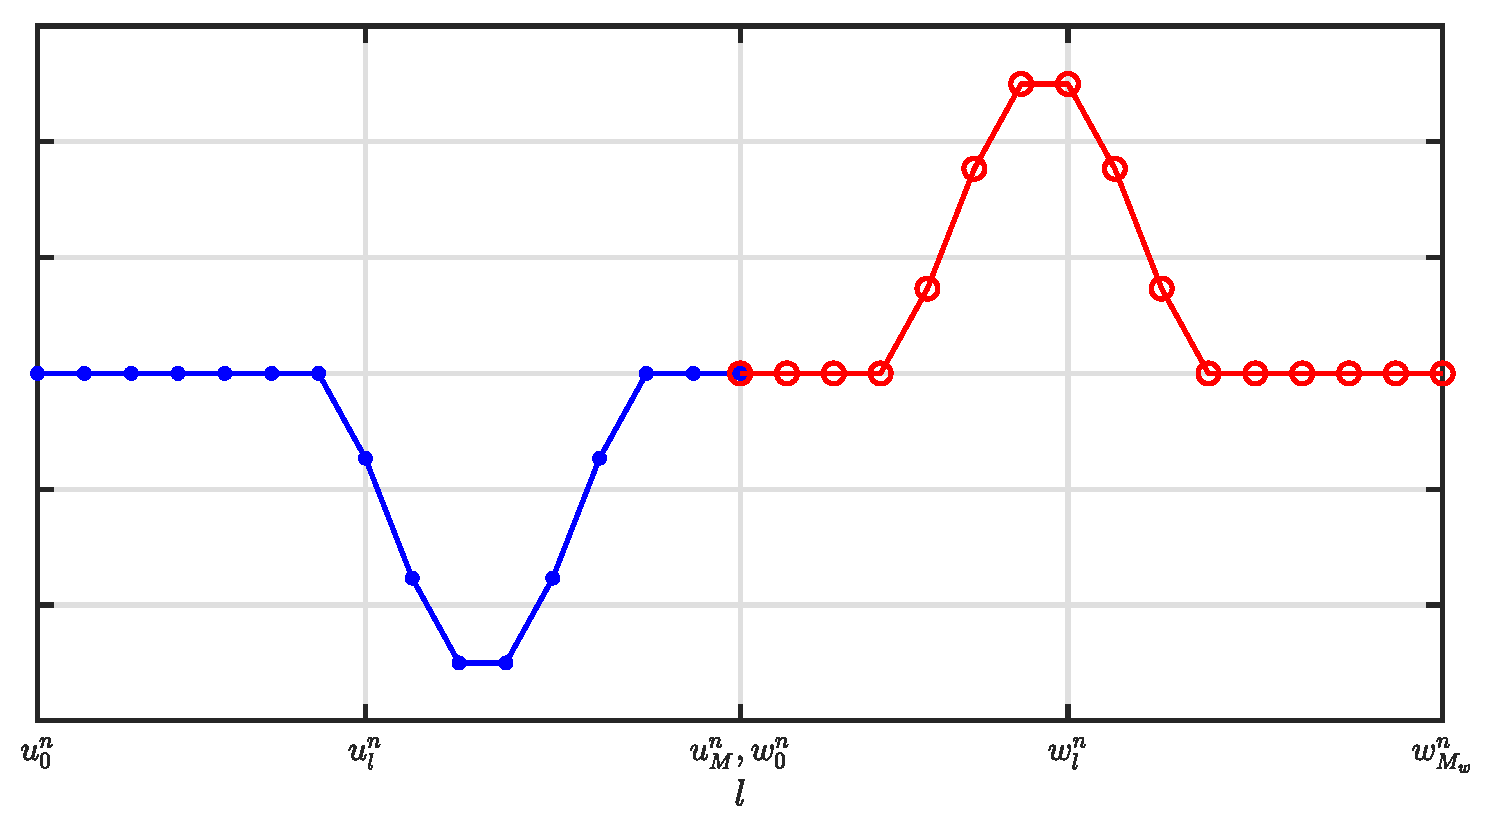
\includegraphics[width=\columnwidth]{twoFreeStrings.eps} }
% \caption{\label{fig:twoFreeStrings}{Two (1D wave) systems connected at one of their boundaries.}}
% \end{figure}
%
\begin{figure}[h]
% \baselineskip=12pt
\figcolumn{
\fig{twoFreeStrings}{\reprintcolumnwidth}{(A)}\label{fig:twoFreeStrings}
\fig{twoFreeStringGridMove}{\reprintcolumnwidth}{(B)}\label{fig:twoFreeStringsGridMove}
\fig{twoFreeStringGridMoveZoomed}{\reprintcolumnwidth}{(C)}\label{fig:twoFreeStringsGridZoomed}
}
\caption{Illustration of the proposed method. (A) Locations of the states of two (1D wave) systems connected at the inner boundary ($N = 30$, $x_{u_M} = x_{w_0}$). (B) When $c$ -- and consequently $h$ -- are decreased and the positions of the grid points change ($N = 30.5$, $x_{u_M} \neq x_{w_0}$). (C) Figure \ref{fig:twoFreeStringsGridMove} zoomed-in around $x_{u_M}$ and $x_{w_0}$. The states at the inner boundaries $u_M$ and $w_0$ are shown together with virtual grid points $u_{M+1}$ and $w_{-1}$. In all figures, the x-axis shows the location (in m) of the respective grid points (fx. $x_{u_l}$), but the $x$ is omitted for brevity.}
\end{figure}
%
The systems can then be connected at the inner boundaries ($u_M$ and $w_0$) using a rigid connection, i.e. \SWcomment[(only valid if $x_{u_M} = x_{w_0}$)],
\begin{equation}\label{eq:rigid}
    u_M^n = w_0^n,\quad \forall n.
\end{equation}
Essentially, the complete system is divided into two separate systems connected at the inner boundary. The system will now be
\begin{equation}
    \begin{cases}\label{eq:systemHalfStrings}
        \delta_{tt}u_l^n = c^2\delta_{xx}u_l^n + J(x_{u_M})F\\
        \delta_{tt}w_l^n = c^2\delta_{xx}w_l^n - J(x_{w_0})F
    \end{cases}
\end{equation}
with spreading operator
\begin{equation}
    J(x_i) =
    \begin{cases}
        \frac{1}{h}, & l = l_i\\
        0,& \text{otherwise}
    \end{cases}
\end{equation}
and the effect of the connection \SWcomment[(``connection force", but not really as it isn't in N)] $F$ (in m$^2$/s$^2$).
%
Expanding the spatial operators in system \eqref{eq:systemHalfStrings} at inner boundaries $u_M^n$ and $w_0^n$, recalling the conditions in  \eqref{eq:halfStringBoundaryCond} and the definition for the virtual grid points needed for the Neumann condition in Eq. \eqref{eq:neumannSolution} yields
\begin{equation}\label{eq:expandedSystem}
    \begin{cases}
        \delta_{tt}u_M^n = \frac{c^2}{h^2}(2u_{M-1}^n-2u_M^n) + \frac{1}{h}F\\
        \delta_{tt}w_0^n = \frac{c^2}{h^2}(2w_1^n-2w_0^n) - \frac{1}{h}F.
    \end{cases}
\end{equation}
Because of Eq. \eqref{eq:rigid}, it is also true that $\delta_{tt}u_M^n = \delta_{tt}w_0^n$, and $F$ can be calculated by setting the \SWcomment[right side of the] equations in \eqref{eq:systemHalfStrings} equal to each other:
\begin{align}
     \frac{c^2}{h^2}(2u_{M-1}^n-2u_M^n) + \frac{1}{h} F&= 
     \frac{c^2}{h^2}(2w_1^n-2w_0^n) - \frac{1}{h} F\nonumber\\
    % \frac{2}{h}F &= \frac{c^2}{h^2}(2w_1^n - 2u_{M-1}^n)\nonumber\\
    F &= h \frac{c^2}{h^2}(w_1^n - u_{M-1}^n)
\end{align}
Substituting this into system \eqref{eq:expandedSystem} after expansion of the second-time derivative yields
\begin{equation}\label{eq:resultOneConnectedPoint}
    \begin{cases}
    u^{n+1}_M = 2u_M^n - u_n^{n-1} + \lambda^2(u_{M-1}^n-2u_M^n+w_1^n)\\
    w^{n+1}_0 = 2w_0^n - w_0^{n-1} + \lambda^2(u_{M-1}^n-2w_0^n+w_1^n)
    \end{cases}
\end{equation}
which, (again, recalling Eq. \eqref{eq:rigid}) are indeed equivalent expressions for the connected point. Here, $w_1^n$ in the first expression acts as virtual grid point $u_{M+1}^n$ and $u_{M-1}^n$ as virtual grid point $w_{-1}^n$, essentially connecting the two systems using the state of one in the update of the other.

\subsubsection{Changing the Grid}
Section \ref{sec:systSetup} describes the case in which the stability condition is satisfied with equality, i.e, when $1/ck$ is an integer and $x_{u_M} = x_{w_0}$ \SWcomment[(read as: the locations of grid points $u_M$ and $w_0$ are identical)]. The locations of the outer boundaries $x_{u_0}$ and $x_{w_{M_w}}$ are fixed, i.e.
\begin{equation}
    x_{u_0}^n = x_{u_0}^0 \quad \text{and}\quad x_{w_{M_w}}^n = x_{w_{M_w}}^0 \quad \forall n.
\end{equation}
If the wave speed $c$ is then decreased, and consequently the grid spacing $h$ according to $h=ck$, all other points move towards their respective outer boundary (see Figure \ref{fig:twoFreeStringsGridMove}). Calculating $h$ this way allows this method to always satisfy the CFL condition in Eq. \eqref{eq:CFL} with equality, as is the case with the previous iteration described in \ref{sec:iterations}.

% \begin{figure}[h]
% \centerline{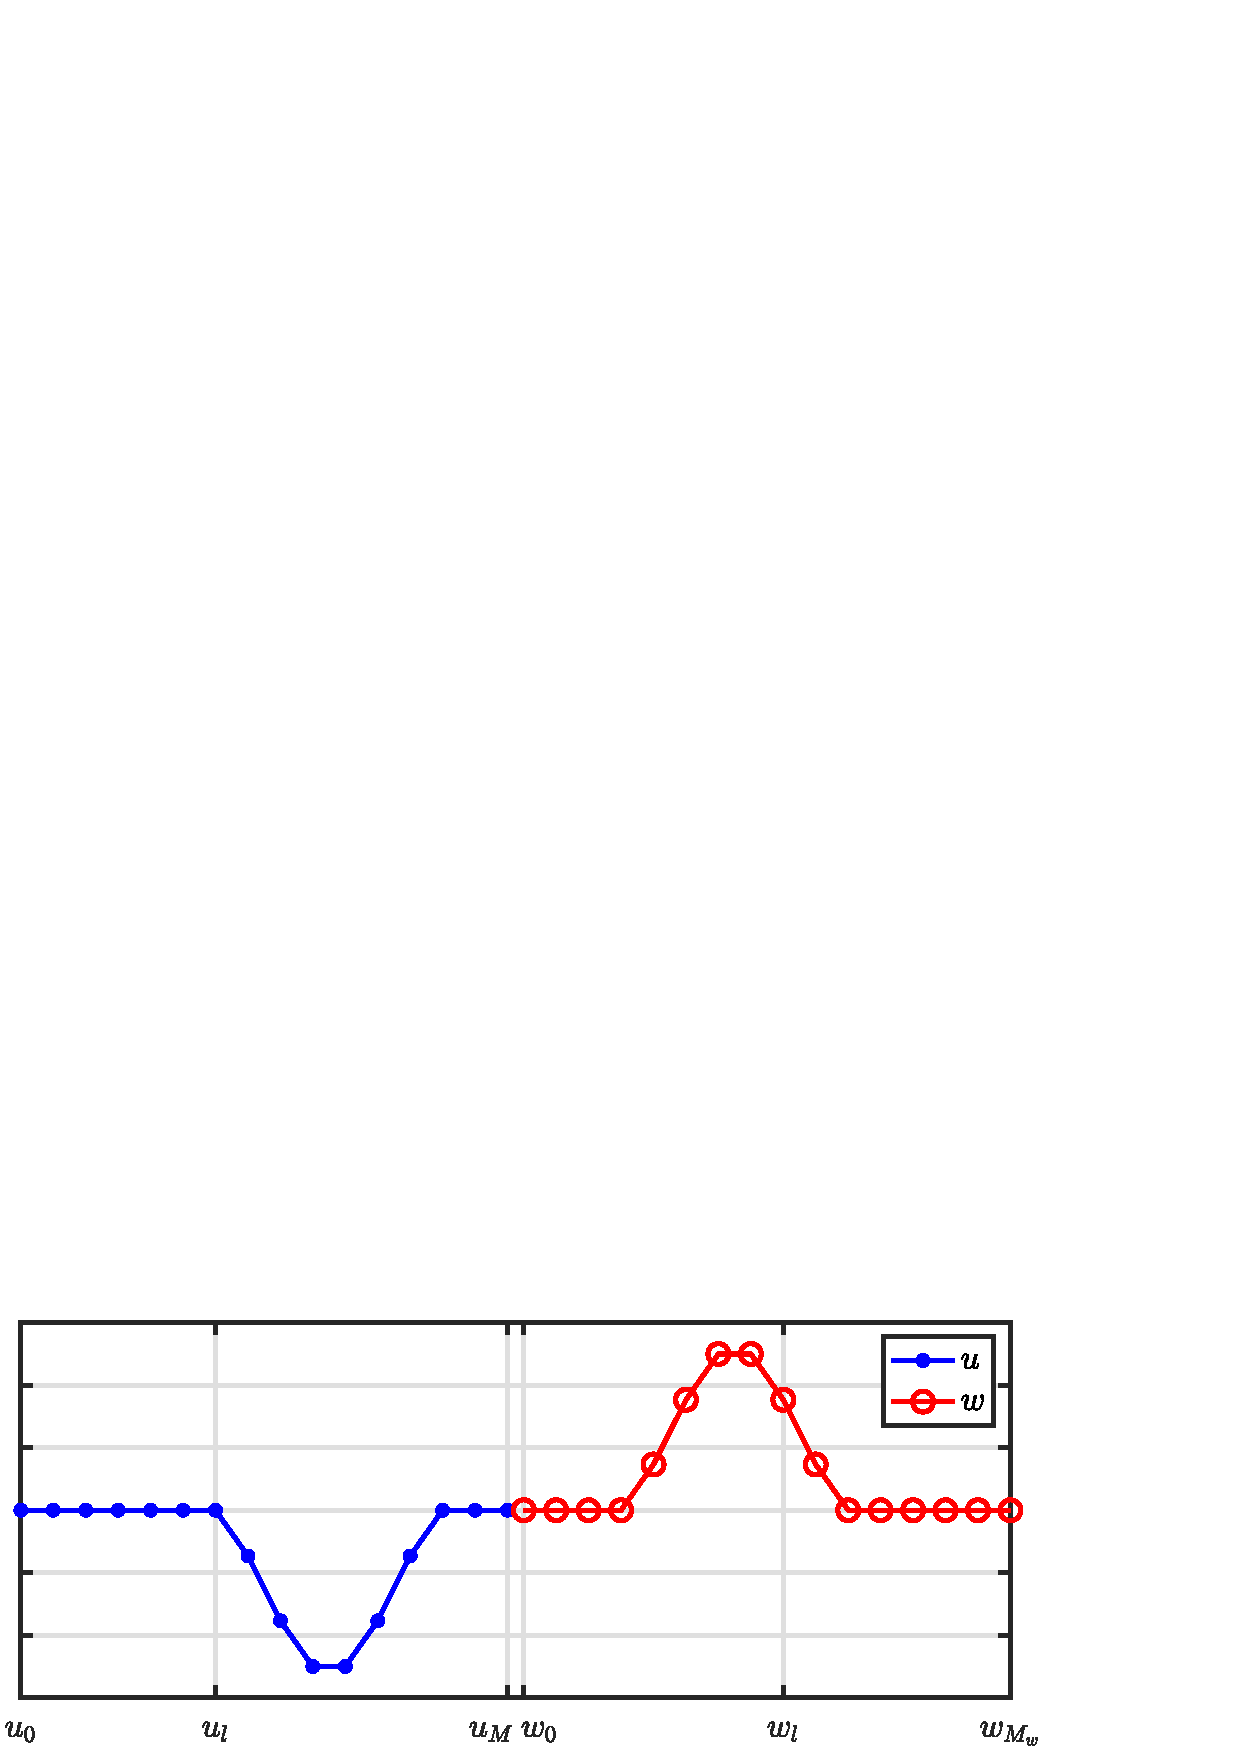
\includegraphics[width=\columnwidth]{twoFreeStringGridMove} }
% \caption{\label{fig:twoFreeStringsGridMove}{When the grid changes ($N = 30.5$). The x-axis shows the location (in m) of the respective grid points (fx. $x_{u_l^n}$), but the $x$ is omitted for clarity.}}
% \end{figure}
%
As mentioned above, the state of $\mathbf{w}$ can be used to calculate the virtual grid point needed at the right boundary of $\mathbf{u}$ and vice versa. If $x_{u_{M+1}} \neq x_{w_1}$ (and thus $x_{w_{-1}} \neq x_{u_{M-1}}$) \SWcomment[$\leftarrow$ I think this is clearer than simply saying $x_{w_0} \neq x_{u_M}$ as these are used in the Eqs. in \eqref{eq:interpolationGeneral} below] an interpolator $I(x_i)$ at location $x_i$ (in m) can be used to calculate the value of this virtual grid point
\begin{subequations}\label{eq:interpolationGeneral}
    \begin{align}
        u_{M+1}^n &= I(x_{u_{M+1}})w_l^n% = (1-\alpha)w_1^n + \alpha w_0^n
        \\
        w_{-1}^n &= I(x_{w_{-1}})u_l^n.% = (1-\alpha)u_{M-1}^n + \alpha u_M^n
    \end{align}
\end{subequations}
% where
% \begin{equation}
%     \alpha = \frac{x_{w_0} - x_{u_M}}{h},
% \end{equation}
% and grid-point locations $x_{u_{M+1}}$ and $w_{-1}$. Note that when $h$ changes the connected points start to move away from each other.
%
If linear interpolator $I_1$ is used, the Eqs. in \eqref{eq:interpolationGeneral} can easily be calculated from known values according to
\begin{subequations}
    \begin{align}
        u_{M+1}^n &= I_1(x_{u_{M+1}})w_l^n = (1-\alpha)w_1^n + \alpha w_0^n
        \\
        w_{-1}^n &= I_1(x_{w_{-1}})u_l^n = (1-\alpha)u_{M-1}^n + \alpha u_M^n
    \end{align}
\end{subequations}
where
\begin{equation}
    \alpha = \frac{x_{w_0} - x_{u_M}}{h}\,.
\end{equation}
Also see Figure \ref{fig:twoFreeStringsGridZoomed}.
% \begin{figure}[h]
% \centerline{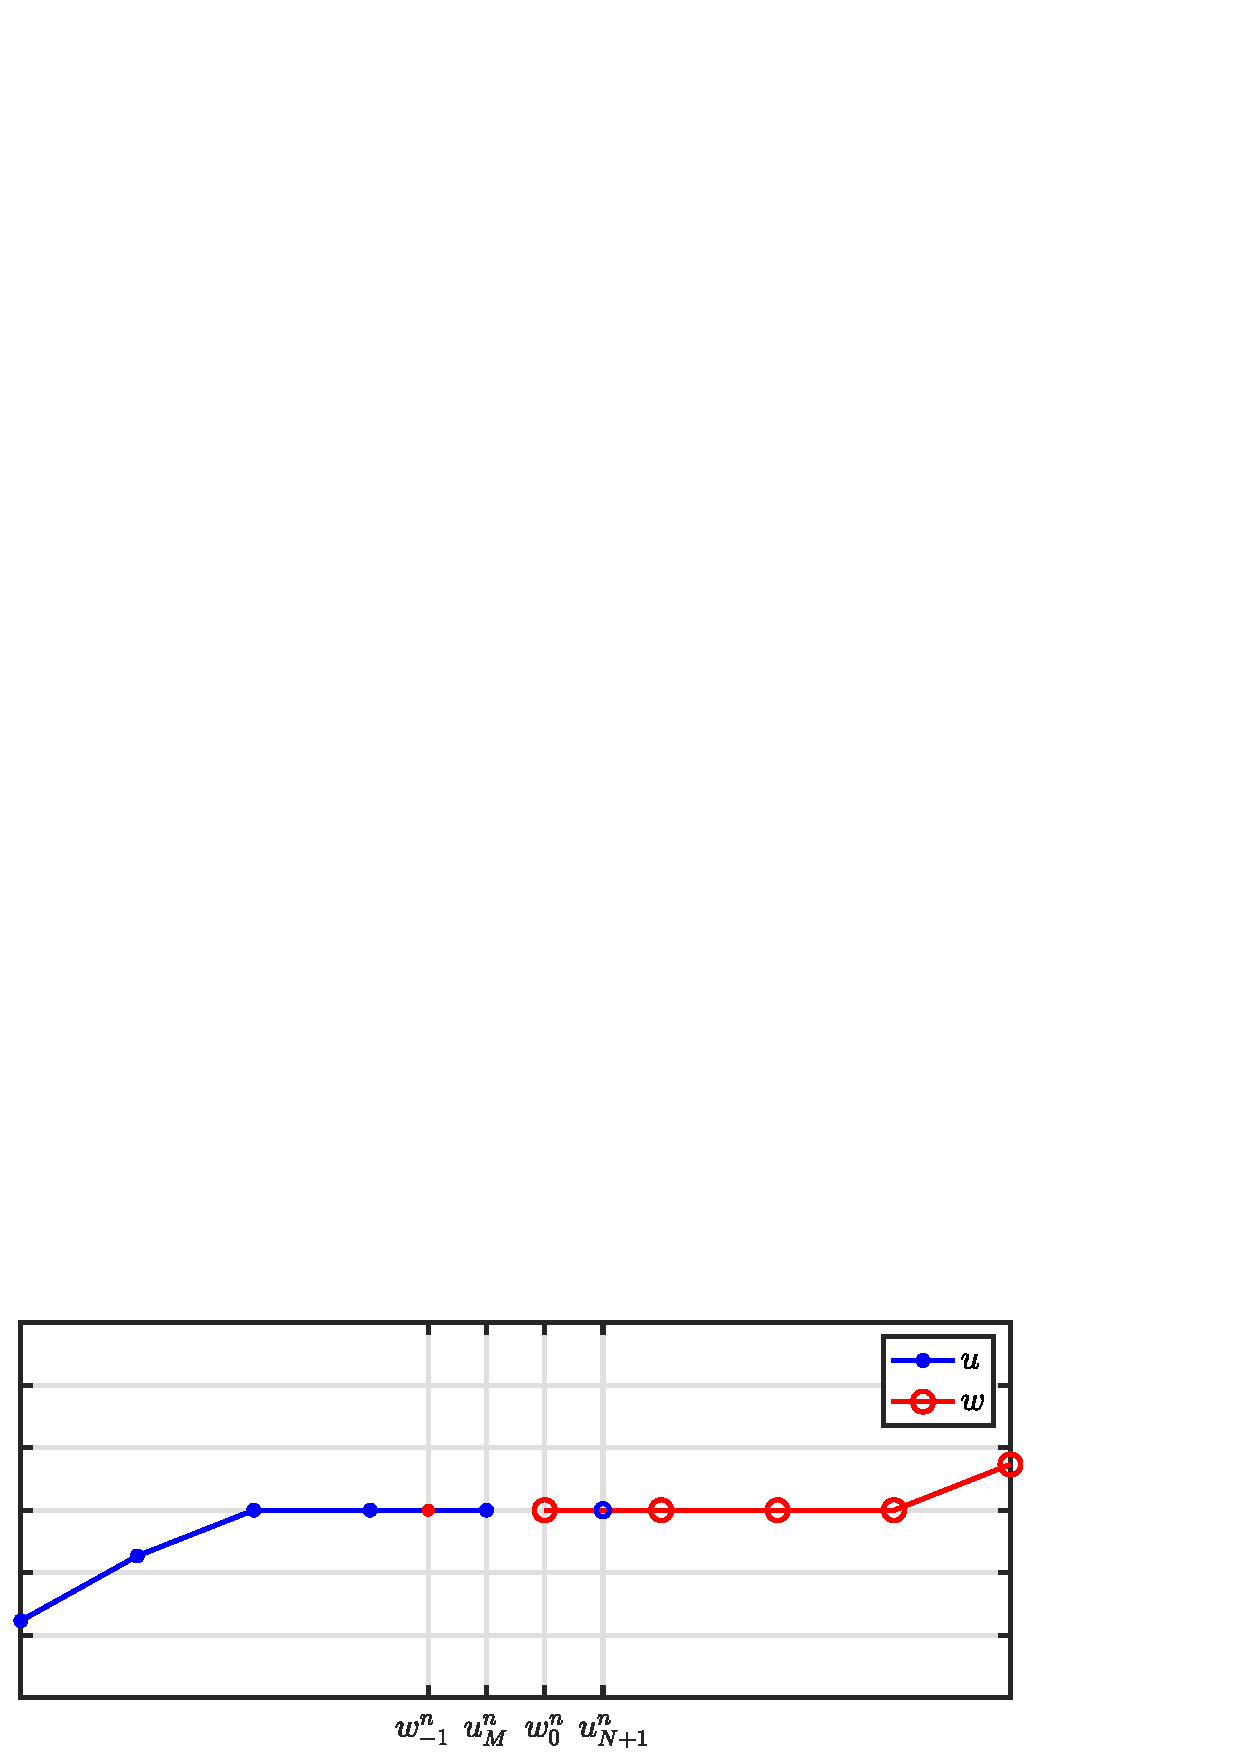
\includegraphics[width=\columnwidth]{twoFreeStringGridMoveZoomed} }
% \caption{\label{fig:twoFreeStringsGridZoomed}{When the grid changes (zoomed). The states at the inner boundaries $u_M$ and $w_0$ are shown together with virtual grid points $u_{M+1}$ and $w_{-1}$.}}
% \end{figure}

Using $I_1$, analysis of the output shows that the expected fundamental frequency is slightly higher when interpolation needs to happen than the one expected when using Eq. \eqref{eq:fundamentalFreq}. Instead of a linear interpolation, the cubic interpolator $I_3$ can be used according to 
\begin{subequations}\label{eq:connectionInterpol}
\begin{align}
    &\begin{aligned}\label{eq:calcUMP1}
        u_{M+1}^n &= I_3(x_{u_{M+1}})w_l^n\\
        &= \alpha_\text{I}w_2^n + \beta_\text{I}w_1^n + \gamma_\text{I}w_0^n + \delta_\text{I} w_{-1}^n
    \end{aligned}\\
    &\ \ \begin{aligned}\label{eq:calcWM1}
        w_{-1}^n &= I_3(x_{w_{-1}})u_l^n \\
        &=\alpha_\text{I} u_{M-2}^n + \beta_\text{I}u_{M-1}^n+ \gamma_\text{I}u_M^n + \delta_\text{I} u_{M+1}^n.
    \end{aligned}
\end{align}
    
\end{subequations}
where
\begin{gather*}
    \alpha_\text{I} = \frac{\alpha(\alpha - 1)(\alpha - 2)}{-6}, \quad \beta_\text{I} = \frac{(\alpha - 1)(\alpha + 1)(\alpha - 2)}{2},\\
    \gamma_\text{I} = \frac{\alpha(\alpha + 1)(\alpha - 2)}{-2}, \quad \text{and} \quad\delta_\text{I} = \frac{\alpha(\alpha + 1)(\alpha - 1)}{6}\,.
\end{gather*}
Treating \eqref{eq:connectionInterpol} as a system of linear equations, the virtual grid points $u_{M+1}^n$ and $w_{-1}^n$ can be solved for using
\begin{equation}\label{eq:linSystSolution}
    \begin{bmatrix}
    u_{M+1}^n \\
    w_{-1}^n
    \end{bmatrix}
    =
     \begin{bmatrix}
         1 & -\delta_\text{I} \\
         -\delta_\text{I} & 1
    \end{bmatrix}^{-1}\begin{bmatrix}
    \alpha_\text{I} w_2^n+ \beta_\text{I}w_1^n + \gamma_\text{I}w_0^n \\
    \alpha_\text{I} u_{M-2}^n + \beta_\text{I}u_{M-1}^n + \gamma_\text{I} u_{M}^n
    \end{bmatrix}.
\end{equation}
% where
% \begin{equation}\nonumber
%     \mathbf{A} = \begin{bmatrix}
%          1 & -\delta_\text{I} \\
%          -\delta_\text{I} & 1
%     \end{bmatrix},
% \end{equation}
% and
% \begin{equation}\nonumber
%     \mathbf{v} = \begin{bmatrix}
%     \alpha_\text{I} w_2^n+ \beta\text{I}w_1^n + \gamma\text{I}w_0^n \\
%     \alpha_\text{I} u_{M-2}^n + \beta\text{I}u_{M-1}^n + \gamma u_{M}^n
%     \end{bmatrix}.
% \end{equation}
As will be shown in Section \ref{sec:results}, cubic interpolation yields the expected fundamental frequency at all times.% also when interpolation needs to happen.

\subsubsection{Adding and removing Grid Points}
The location at where points are added and removed greatly influences the behaviour of the system, especially in the higher frequencies (see Section \ref{sec:results}). The best behaviour is obtained when the location is as close to a boundary as possible. Using a fractional $N$, consider grid functions $u_l^n$ and $w_l^n$ as described before, but now with
\begin{equation}\label{eq:Mdefinition}
   M = \text{floor}(N) - 1 \quad\text{and}\quad M_w = 1. 
\end{equation}
This results in grid function $w_l^n$ only having one moving point $w_0^n$, the boundary at $w_1^n$ and virtual grid point $w_2^n$ (see Figure \ref{fig:addingPoint}). Condition \eqref{eq:halfStringBoundaryCondDirichlet} can be extended at the right boundary to be simply supported
\begin{equation}
    w_{M_w}^n = \delta_{xx}w_{M_w}^n = 0, \quad \text{(simply supported)}
\end{equation}
which after expansion and knowing $M_w = 1$ can be solved to \SWcomment[(similarly to Eq. \eqref{eq:neumannSolution})]
\begin{equation}\label{eq:simplySupportedSolved}
    w_1 = 0 \quad \text{and} \quad w_2^n = -w_0^n.
\end{equation}
This simplifies Eq. \eqref{eq:calcUMP1} to
\begin{equation}
    u_{M+1}^n = (\gamma_\text{I} - \alpha_\text{I})w_0^n + \delta_\text{I}w_{-1}^n,
\end{equation}
and can be inserted in Eq. \eqref{eq:linSystSolution}. 

When $c$, and consequently $h$, is decreased and the boundary points surpass the virtual points (i.e. $x_{u_M} \leq x_{w_{-1}}$ and $x_{u_{M+1}} \leq x_{w_0}$) and $M^n > M^{n-1}$ (calculated using \eqref{eq:Mdefinition}), a point approximating $u_{M+1}^n$ is added at the right boundary of $\mathbf{u}^n$ (for both time indices $n$ and $n-1$)
\begin{equation}\label{eq:addingPoint}
       \mathbf{u}^n = [(\mathbf{u}^n)^T, I_3'(x_{u_{M+1}})\mathbf{v}^n]^T
\end{equation}
where
\begin{equation*}
\mathbf{v}^n = [u_{M-1}^n, u_M^n, w_0^n, w_1^n]^T, 
\end{equation*}
and
\begin{equation}\label{eq:customIp}
    I_3' = \begin{bmatrix} -\frac{\alpha'(\alpha'+1)}{(\alpha'+2)(\alpha'+3)} &\frac{2\alpha'}{\alpha'+2} &\frac{2}{\alpha'+2} 
    &-\frac{2\alpha'}{(\alpha'+3)(\alpha'+2)}
    \end{bmatrix},
\end{equation}
\SWcomment[(created using 4-point Lagrange interpolation)] with
\begin{equation}
    \alpha' = \frac{x_{w_0} - (x_{u_M} + h)}{h}\ .\nonumber
\end{equation}
See Figure \ref{fig:addingPoint}.
% Note that this operation is done for both time indices $n$ and $n-1$.

\begin{figure}[ht]
%% \reprintcolumnwidth is the same in preprint and reprint for
%% ease of use for authors:
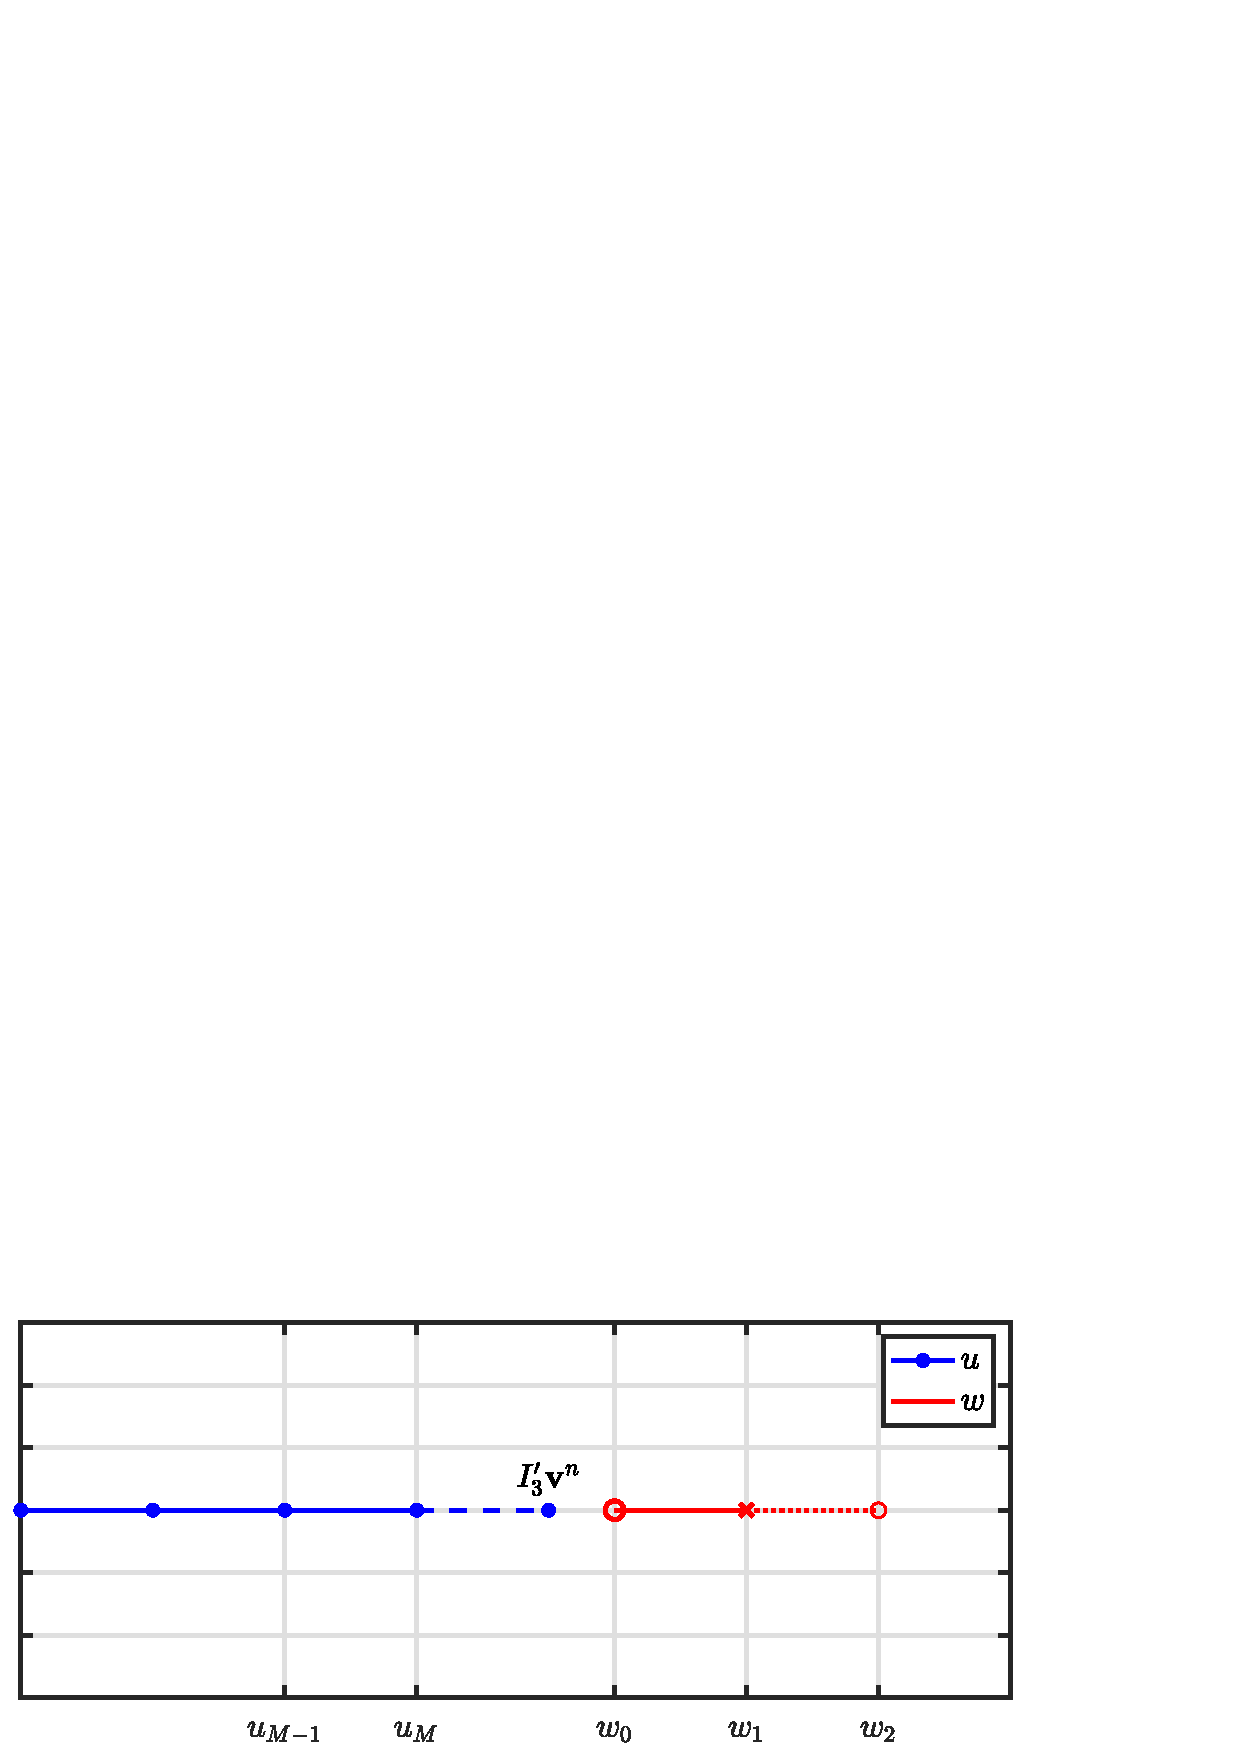
\includegraphics[width=\reprintcolumnwidth]{addingGridPoint2}
\caption{\label{fig:addingPoint}{The system with $M = N-1$ and $M_w = 1$. System $w$ only has one moving point $w_0$, the boundary $w_1$ and virtual grid point $w_2$ defined by condition \eqref{eq:simplySupportedSolved}. The figure shows the moment when a point is added to $\mathbf{u}$ at location $x_{u_M} + h$ in Eq. \eqref{eq:addingPoint}. This figure shows an extreme case where this location is far from $x_{w_0}$, i.e., $\alpha' \not\approx 0$ in Eq. \eqref{eq:customIp}.}}
\end{figure} 

As $\alpha'$ in Eq. \eqref{eq:customIp} is expected to be close to zero \SWcomment[maybe explain that at low parameter variations this happens?], the third term in $\mathbf{v}^n$ is expected to have the biggest contribution to the newly added point. This makes sense by looking at Figure \ref{fig:twoFreeStringsGridZoomed}, as exactly when boundary point $w_0^n$ surpasses virtual point $u_{M+1}^n$, these are going to be close to overlapping.

Removing grid points happens when $c$, and consequently $h$, is increased and the boundary points surpass the virtual points (i.e. $x_{u_M} \geq x_{w_{-1}}$ and $x_{u_{M+1}} \geq x_{w_0}$) and $N^n < N^{n-1}$. Compared to adding grid points, removing them is slightly easier where points are simply removed from the end of $\mathbf{u}$
\begin{equation}\label{eq:removingPoint}
    \mathbf{u}^n = [u_0^n, u_1^n ..., u_{M-1}^n]^T. 
\end{equation}


\section{Results}\label{sec:results}
This section shows the analysis of the system presented in the previous section and its behaviour.

\subsection{Static}
In order to determine whether the proposed method yields an output with the correct frequency content, a spectrum is taken of the system's output. The system with $N=15.5$ at a sample rate of $f_\text{s} = 44100$ Hz is compared to the same system with $f_\text{s} = 88200$ Hz resulting in $N=31$ for the same $f_0$ according to Eq. \eqref{eq:fundamentalFreq}. See Figure \ref{fig:spectra}.

is achieved when the system is static, but when interpolation needs to be used (i.e., $\alpha\neq 0$ in Eq. \eqref{eq:connectionInterpol}) the spectrum is plotted 

\begin{itemize}
    \item Comparing static linear and cubic interpolation ($N = 30.5$)
    \item Comparing full-grid interpolation at insane sample rates
\end{itemize}


\begin{figure}[ht]
%% \reprintcolumnwidth is the same in preprint and reprint for
%% ease of use for authors:
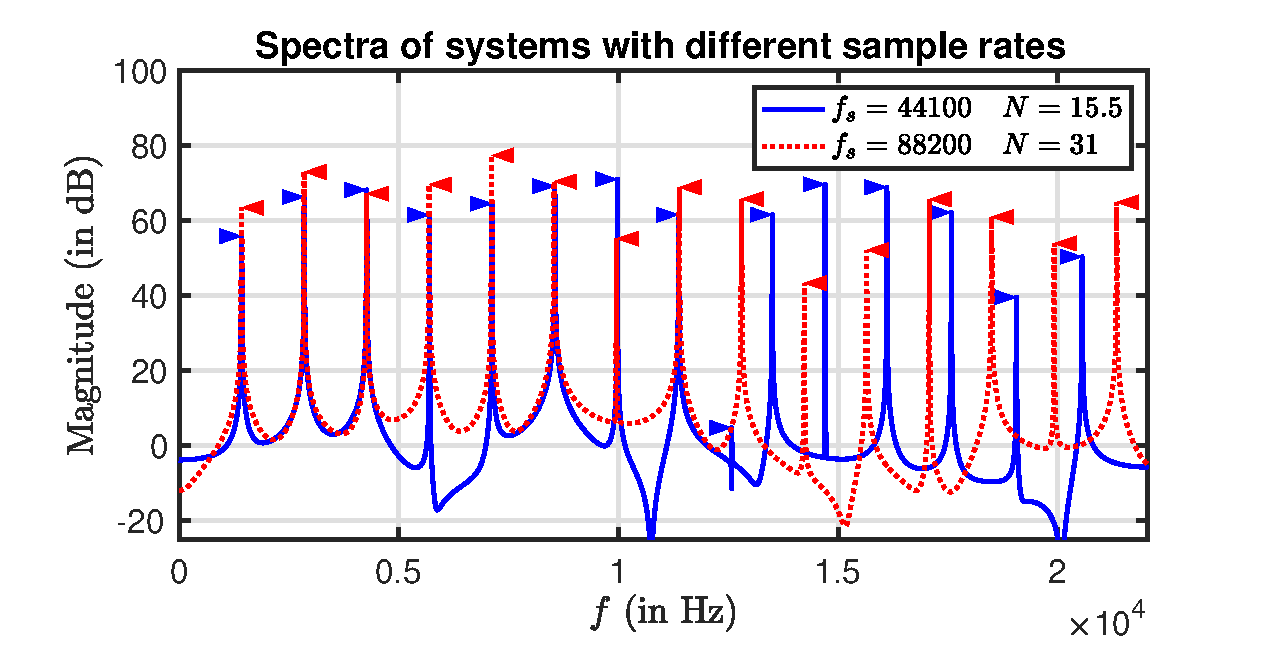
\includegraphics[width=\reprintcolumnwidth]{spectraDoubleSampleRate.eps}
\caption{\label{fig:spectra}{A system with $N = 15.5$ at $f_\text{s} = 44100$}}
\end{figure} 


\subsection{Dynamic}

\begin{figure}[ht]
%% \reprintcolumnwidth is the same in preprint and reprint for
%% ease of use for authors:
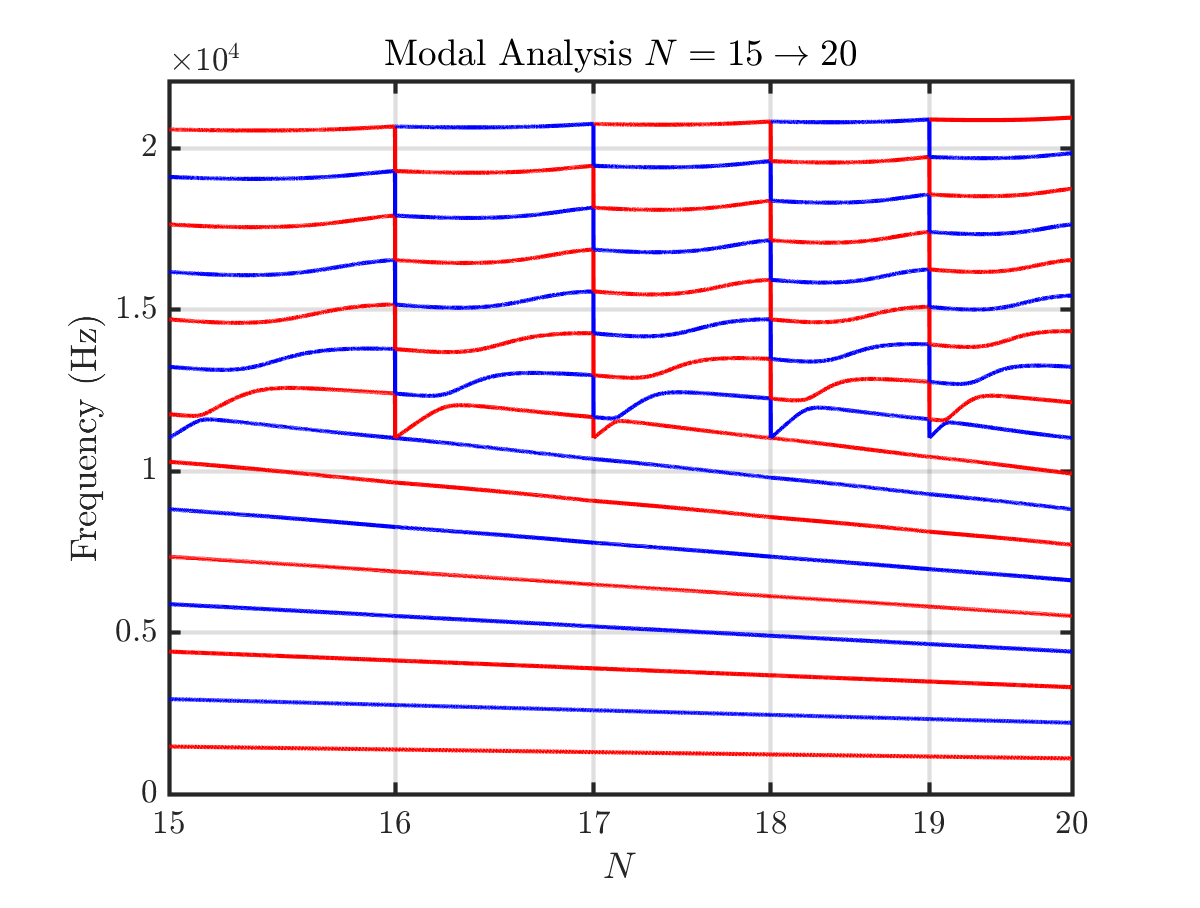
\includegraphics[width=\reprintcolumnwidth]{modesAddPointsAtRightBound.eps}
\caption{\label{fig:addingPoint}{Modal analysis}}
\end{figure} 

\begin{figure}[ht]
%% \reprintcolumnwidth is the same in preprint and reprint for
%% ease of use for authors:
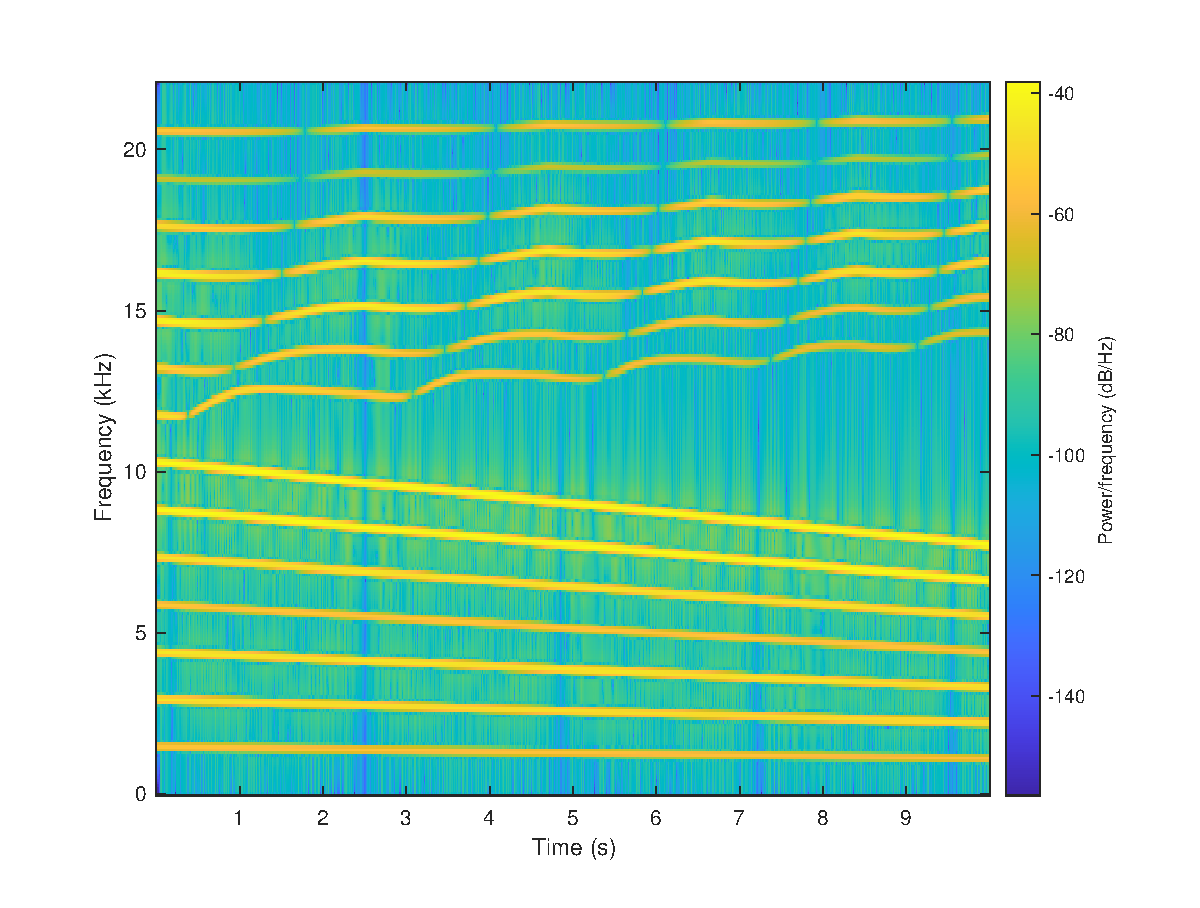
\includegraphics[width=\reprintcolumnwidth]{specAddPointsAtRightBound.eps}
\caption{\label{fig:addingPoint}{System output}}
\end{figure} 

\section{Discussion}
Applications could be non-linear systems where parameters are modulated based on the state of the system. 

The proposed method does not provide the exact solution to the problem, but does circumvent the need for upsampling and higher orders of computations necessary to approximate this solution. Even though interpolation needs to happen, the drawbacks of full-grid interpolation can be avoided by not `listening' to the location where points are added but rather closer to the boundary. If one wants to listen to the center, the location where points are added or removed can easily be changed.


 frequency domain, the locations of the partials comparing the discrete 1D wave with $N = 30.5$ and $f_\text{s} = 44100$ (interpolation needs to happen) with $N = 61$ and $f$ 

If the amount that a parameter changes within a small enough period of time (give values here, hopefully referring back to the results) the fact that points are added at a specific location (rather than distributed over the grid) will not matter as... 



\SWcomment[Notes (warning, very pretentious):] The aforementioned drawbacks of the method are eclipsed by the advantages it brings in terms of dynamic parameter changes and quality improvements. 

\appendix
\section{Iterations}\label{app:A}
In this appendix, some iterations done over the course of this project will be shown in more detail. In the following, the 1D wave equation with a wave speed of $c = 1470$ m/s, a length of $L = 1$ m, Dirichlet boundary conditions and a sample rate of $f_\text{s} = 44100$ Hz is considered, and -- through Eq. \eqref{eq:compactLambda} -- satisfies the CFL condition with equality. These values result in $N = 30$, or a grid of 31 points including the boundaries. Then, the wave speed is decreased to $c \approx 1422.6$ m/s, i.e., the wave speed that results in $N=31$ and satisfies the stability condition with equality again. 

\subsection{Full-Grid Interpolation}
One way to go from one grid to another is performing a full-grid interpolation \cite[Chap. 5]{bilbao2009}. If the number of points changes according to Eq. \eqref{eq:orderOfCalcGrid}, i.e., if $N^n \neq N^{n-1}$ the full state of the system ($u_l^n, u_l^{n-1}\ \forall l$)  can be interpolated to the new state. See Figure \ref{fig:fullGrid}. 

\begin{figure}[h]
%% \reprintcolumnwidth is the same in preprint and reprint for
%% ease of use for authors:
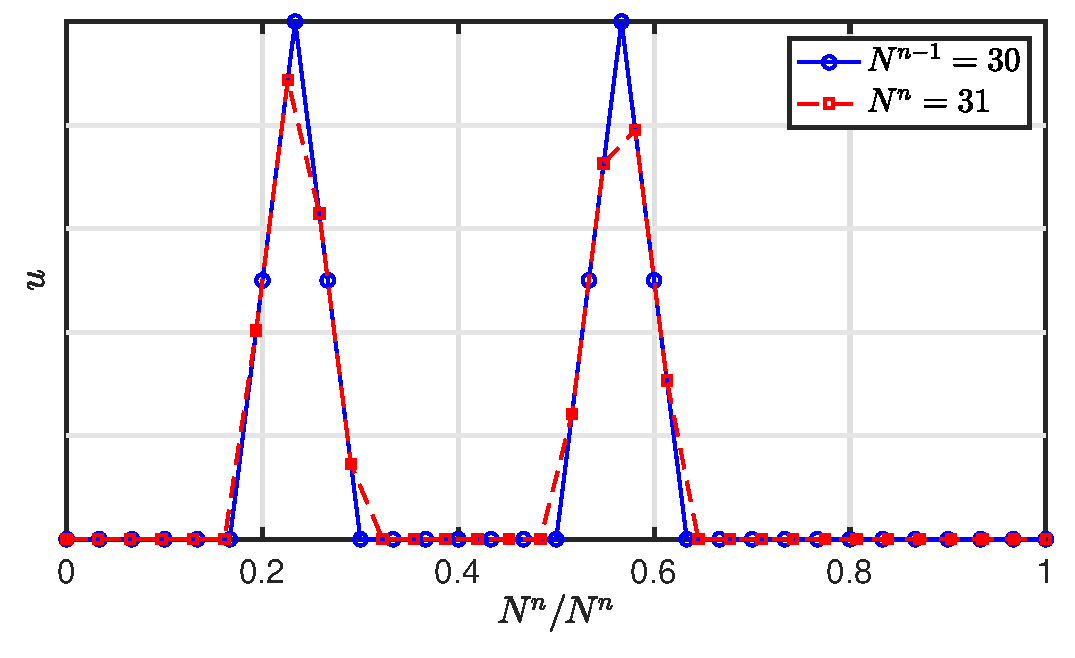
\includegraphics[width=\reprintcolumnwidth]{fullGrid}
\caption{\label{fig:fullGrid}{Upsampling $u$ (with an arbitrary state) using (linear) full-grid interpolation with $N^{n-1} = 30$ and $N^n = 31$. The horizontal axis is normalised with respect to $N^n$.}}
\end{figure} 

An issue that arises using this method is that the Courant number $\lambda$ will slightly deviate from the CFL condition as $c$ changes. Using Eq. \eqref{eq:compactLambda} with $L/ck$ approaching $31$ (from below), the minimum value of $\lambda \approx 30/31 \approx 0.9677$.
%\footnote{Eq. \eqref{eq:orderOfCalcGrid} can be compactly rewritten as $\lambda = \frac{ck}{L}\cdot \text{floor}\left(\frac{L}{ck}\right)$. As $L/ck$ approaches $31$ (from below), $\lambda \approx \frac{30}{31}$.}
This, employing Eq. \eqref{eq:fmax}, has a maximum frequency output of $f_\text{max} \approx 18,475$ Hz. 
%For slightly lower values of $c$, $N = 31$ and $\lambda \approx 1$. 
The Courant number will deviate more for higher values of $c$ and thus lower values for $N$ -- for instance, if $N$ approaches $11$ (from below), $\lambda \approx 10/11 \approx 0.9091$ and $f_\text{max} \approx 16,018$ Hz.

Another problem with full-grid interpolation, is that it has a low-passing effect on the system state, and thus on the output sound. %Figure \ref{fig:fullGrid} shows the biggest changes are in the state are at the locations with the biggest difference between the states of consecutive grid points.
Furthermore, this state-interpolation causes artefacts or `clicks' in the output sound as the method causes sudden variations in the states.  

All the aforementioned issues could be solved by using a (much) higher sample rate and thus more grid points, but this would render this method impossible to work in real time.

\subsection{Adding and removing Points at the Boundary}\label{sec:addAtBoundary}
To solve the issues exhibited by a full-grid interpolation, points can be added and removed at a single location and leave most points unaffected by the parameter changes. A good candidate for a location to do this is at a fixed (Dirichlet) boundary. The state $u$ at this location is always $0$ so points can be added smoothly. 

As $c$ decreases, $h$ can be calculated according to Eq. \eqref{eq:orderOfCalcGrid} and decreases as well.

This has a physical analogy with tuning a guitar string. Material enters and exits the neck (playable part of the string) at the nut, which in discrete time means grid points appearing and disappearing at one boundary.

To yield smooth changes between grid configurations, an interpolated boundary has been developed, the possibility of which has been briefly mentioned in \cite[p. 145]{bilbao2009}. The Dirichlet condition in Eq. \eqref{eq:contDirichlet} can be extended to be the simply supported boundary condition:
\begin{equation}
    u(x, t) = \frac{\partial^2}{\partial x^2}u(x, t) = 0 \quad \text{where} \quad x = 0, L,
\end{equation}
or, when discretised,
\begin{equation}\label{eq:simplySupportedDiscrete}
    u_l^n = \delta_{xx}u_l^n = 0, \quad \text{where} \quad l = 0, N.
\end{equation}
This means that on top of that the state of the boundary should be $0$, the curvature around it should also be $0$. One can again solve for the virtual grid points at the boundary locations, yielding
\begin{equation}
    u_{-1}^n = -u_1^n \quad \text{and} \quad u_{N+1}^n = -u_{N-1}^n.
\end{equation}
This is visualised in Figure \ref{fig:simplySupportedBound}.

\begin{figure}
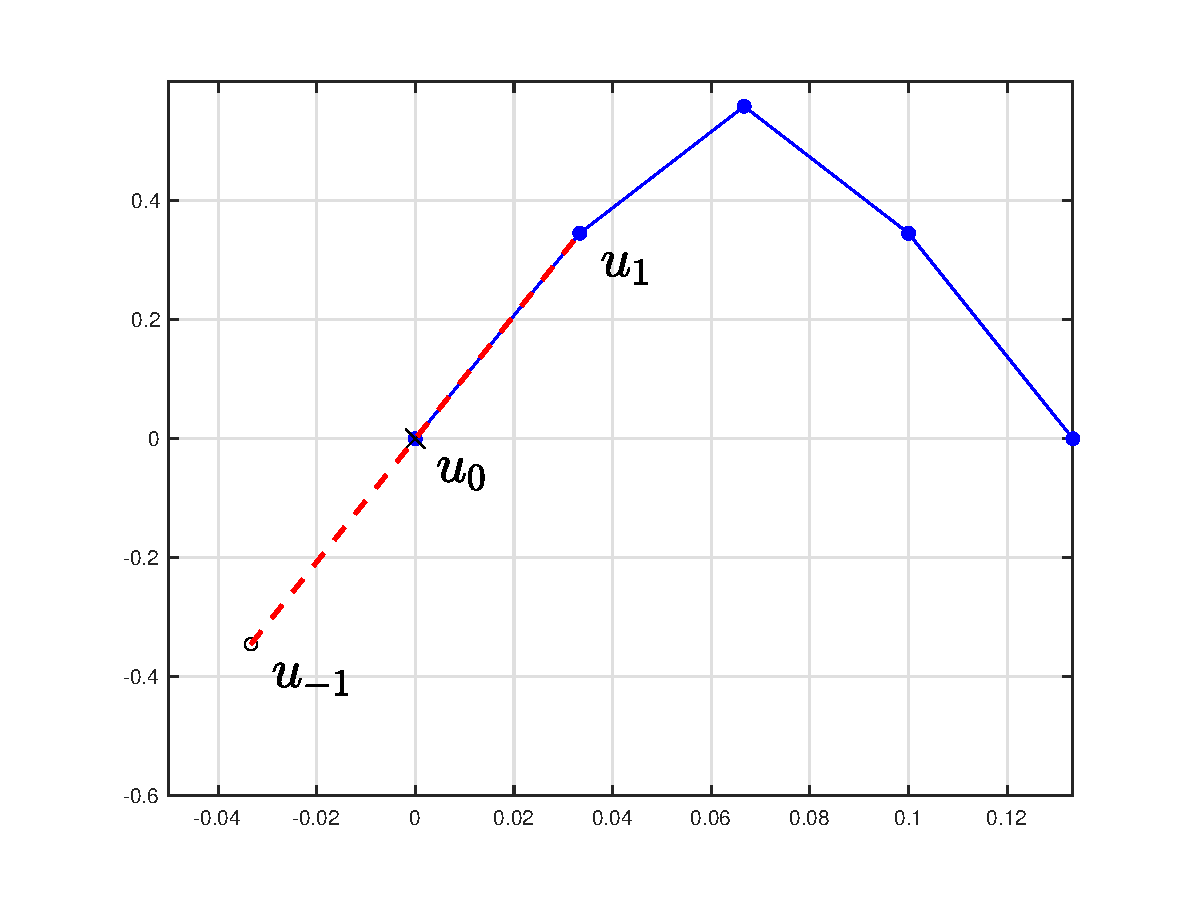
\includegraphics[width=\reprintcolumnwidth]{simplySupportedBoundary}
\caption{\label{fig:simplySupportedBound}{The simply supported boundary condition: both the state and the curvature at the boundary -- at $l=0$ -- should be $0$.}}
\end{figure} 

If the flooring operation in Eq. \eqref{eq:numberOfPoints} is removed this introduces a fractional number of grid points.


The by-product of using a fractional $N$ this is that the CFL condition in \eqref{eq:CFL} can now always be satisfied with equality no matter what the wave speed is.

An issue with this method is that removing points is much harder than adding.

their interactions change through a change in the grid spacing and wave speed. This interaction, though, is defined by $\lambda$ which 

\begin{figure}
%% \reprintcolumnwidth is the same in preprint and reprint for
%% ease of use for authors:
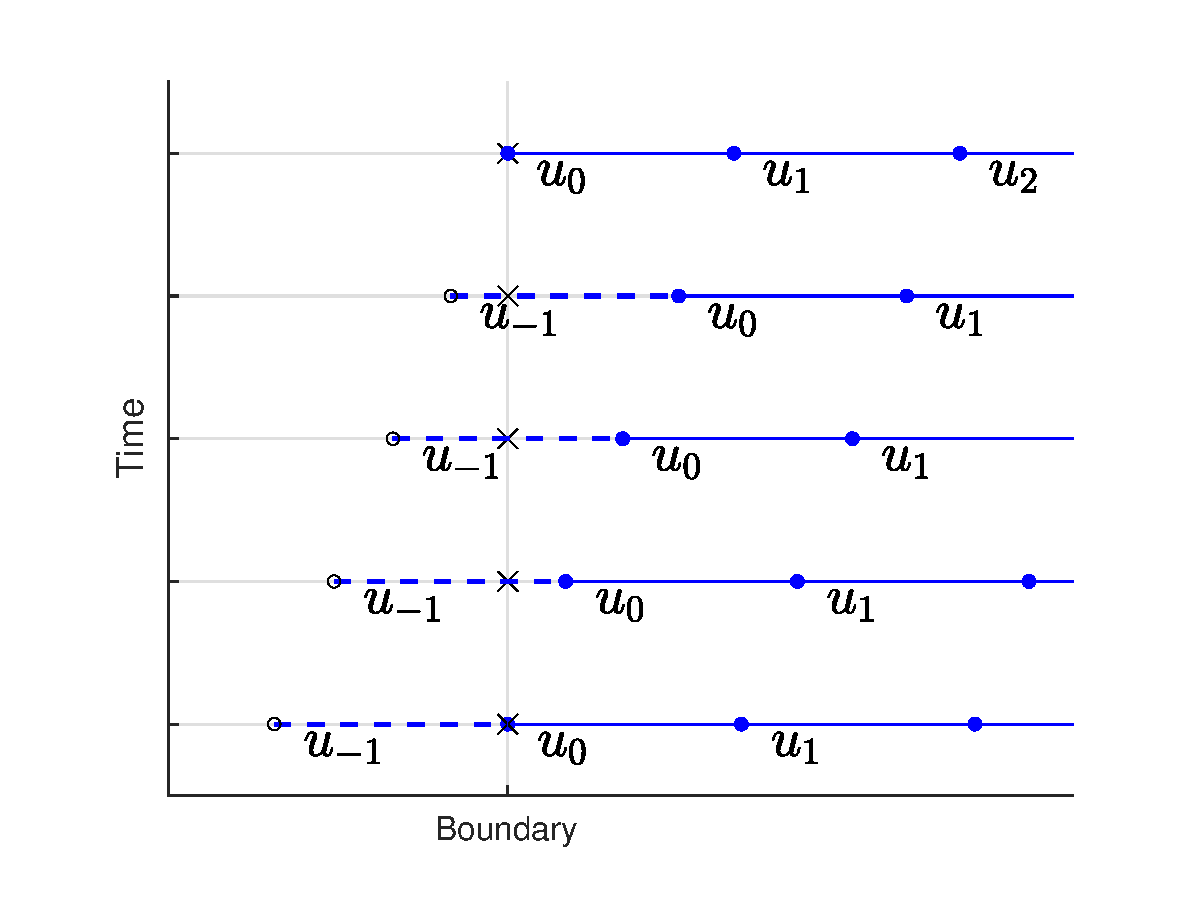
\includegraphics[width=\reprintcolumnwidth]{boundaryGrid}
\caption{\label{fig:changingBoundary}{The grid changing over time}}
\end{figure} 

% \subsubsection{\SWcomment[If the above iterations need to be summarised:]}
\bibliography{myBib}
\end{document}




